\input sys/inputs.tex

\begin{document}

\bigheading{Dálniční fúze}

% \info{task_name}{infile}{outfile}{points}{timelimit}{memlimit}
% leave this values, if you are not interested
\info{networks}{stdin}{stdout}{100}{400 ms}{32 MiB}

V království Bajtozemě\footnote{Poslední dobou komolené také jako \textit{Bojte se mě!}}
mají kromě jiného dvě dálniční sítě,
které jsou poskytovány dvěma společnostmi: Rudá a Modrá.
Obě sítě se skládají z jednobodových křižovatek a z úseček spojucjících
některé dvojice křižovatek. Žádné dvě úsečky se nekříží ani nedotýkají jinde než
v křižovatkách. Obě sítě jsou souvislé, tedy každé dvě křižovatky z jedné sítě
jsou spojené nějakou posloupností navazujících úseček. Navíc jsou oba systémy
disjunktní, jinými slovy žádná křižovatka neleží v obou sítích.
Po nátlaku z Hradu se společnosti nedobrovolně rozhodly,
že spojí své dálniční sítě vybudováním jedné nové úsečky mezi křižovatkou
Rudých a křižovatkou Modrých. Nová úsečka nesmí protínat žádnou jinou úsečku.

\heading{Úloha}
Napište program, který nalezne nějakou vyhovující úsečku.

\heading{Vstup}
Vstup začíná popisem Rudé sítě a pokračuje popisem Modré sítě.

První řádek popisu sítě obsahuje dvě celá čísla $N$ ($2 \leq N \leq 20\,000$) a
$M$ ($1 \leq M \leq 70\,000$). $N$ je počet křižovatek v síti a $M$ je počet
úseček. $i$-tý z následujících $N$ řádků obsahuje dvě celá čísla $x$ a $y$
($-1\,000\,000 \leq x,y \leq 1\,000\,000$), což jsou souřadnice $i$-té křižovatky.
Potom následuje $M$ řádků obsahujících dvě celá čísla $p$ a $q$
($1\leq p \neq q \leq N$), popisující úsečku spojující křižovatky $p$ a $q$.

\bigskip
Ve $30\%$ vstupů počet křižovatek ani počet úseček v žádné síti nepřesáhne $3\,000$.

\heading{Výstup}
První a jediný řádek výstupu obsahuje dvě celá čísla $u$ a $v$,
čísla křižovatek, které nově vybudovaná úsečka propojí.
Přesněji, $u$ je číslo křižovatky Rudých a $v$ je číslo křižovatky Modrých.
Úsečka s koncovými body $u$ a $v$ nesmí křížit žádnou jinou ze stávajících úseček.
Pokud existuje více řešení, může váš program vypsat libovolné z nich,
nezáleží na tom které.

\heading{Příklady}

\sampleIN
5 6
0 3
1 1
6 0
5 3
9 8
1 2
1 3
4 3
3 5
1 5
2 3
4 4
6 4
4 4
4 2
2 3
1 2
4 2
2 3
3 4
\sampleOUT
5 1
\sampleCOMMENT

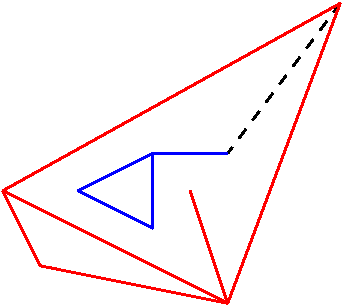
\includegraphics[height=4cm]{img/fig11.pdf}
\sampleEND

\end{document}
